\documentclass{article}
\usepackage{algorithms_in_data_mining}

\begin{document} %
\lecture{6}{SVD and PCA}{Edo Liberty}

\section{Singular Value Decomposition (SVD)}

We will see that any matrix $A \in \R^{m \times n}$ (w.l.o.g. $m \le n$) can be written as 
\begin{eqnarray}
A &=& \sum_{\ell=1}^{m} \sigma_{\ell} u_{\ell} v_{\ell}^{T}\\
&\forall \;\; \ell& \sigma_\ell \in \R,  \;\; \sigma_\ell \ge 0\\
&\forall \;\; \ell, \ell'&  \langle u_{\ell}, u_{\ell'} \rangle=  \langle v_{\ell}, v_{\ell'} \rangle = \delta(\ell,\ell')
\end{eqnarray}
%
To prove this consider the matrix $AA^{T} \in \R^{m\times m}$.
Set $u_\ell$ to be the $\ell$'th eigenvector of $AA^{T}$.
By definition we have that $AA^{T}u_\ell = \lambda_\ell u_\ell$.
Since $AA^{T}$ is positive semidefinite we have $\lambda_\ell \ge 0$.
Since $AA^{T}$ is symmetric we have that $\forall \;\; \ell, \ell' \;  \langle u_{\ell}, u_{\ell'} \rangle = \delta(\ell,\ell')$.
Set $\sigma_\ell = \sqrt{\lambda_\ell}$ and $v_\ell = \frac{1}{\sigma_\ell}A^{T}u_{\ell}$.
Now we can compute the following:
\[
\langle v_{\ell}, v_{\ell'} \rangle =  \frac{1}{\sigma^{2}_\ell}u_{\ell}^{T}AA^{T}u_{\ell} =   \frac{1}{\sigma_{\ell}^{2}}\lambda_\ell  \langle u_{\ell}, u_{\ell'} \rangle = \delta(\ell,\ell')
\]
%
We are only left to show that $A = \sum_{\ell=1}^{m} \sigma_{\ell} u_{\ell} v_{\ell}^{T}$.
To do that we examine the norm or the difference multiplied by a test vector $w = \sum_{i=1}^{m} \alpha_i u_i$.
\begin{eqnarray*}
|| w^{T}(A - \sum_{\ell=1}^{m} \sigma_{\ell} u_{\ell} v_{\ell}^{T})|| &=& || (\sum_{i=1}^{m}\alpha_i u^{T}_{i})(A - \sum_{\ell=1}^{m} \sigma_{\ell} u_{\ell} v_{\ell}^{T})|| \\
&=& || (\sum_{i=1}^{m}\alpha_{i} u^{T}_{i}A - \sum_{i=1}^{m}\sum_{\ell=1}^{m} \delta(i,\ell) \alpha_i \sigma_{\ell} v_{\ell}^{T}|| \\
&=& || (\sum_{i=1}^{m}\alpha_{i} \sigma_{i} v^{T}_{i} - \sum_{i=1}^{m} \alpha_i \sigma_{i} v_{i}^{T}|| = 0
\end{eqnarray*}
%
The vectors $u_\ell$ and $v_{\ell}$ are called the left and right singular vectors of $A$ and $\sigma_\ell$ are the singular vectors of $A$.
It is costumery to order the singular values in descending order $\sigma_1 \ge \sigma_2, \ldots , \sigma_m \ge 0$.
\begin{center}
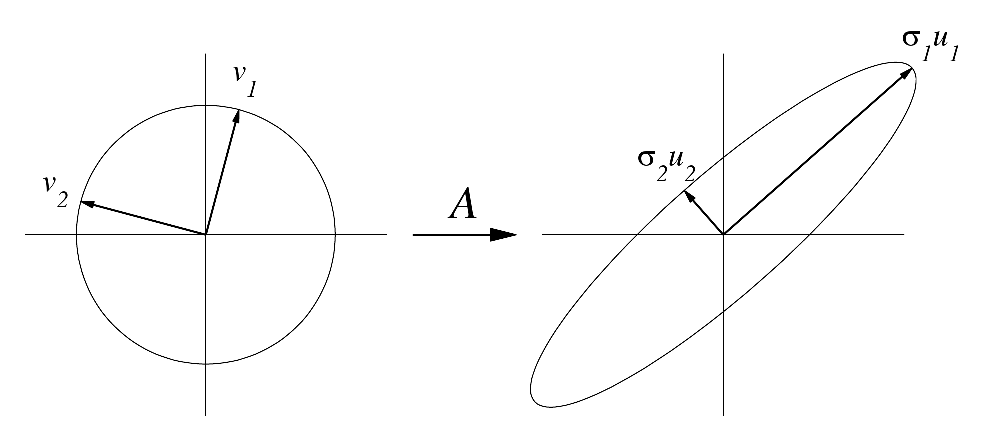
\includegraphics[width=0.6\textwidth]{06_images/SVDgeometry.eps}
\end{center}

\section{Rank-k approximation in the spectral norm}
The following will claim that the best approximation to $A$ by a rank deficient 
matrix is obtained by the top singular values and vectors of $A$. More accurately:
\begin{fact}
Set
\begin{equation*}
A_{k} = \sum_{j=1}^{k} \sigma_{j} u_{j} v_{j}^{T}.
\end{equation*}
Then,
\begin{equation*}
\min_{\substack{B \in \mathbb{R}^{m \times n} \\
\operatorname{rank}(B) \leq k}} \norm{A-B}_{2} = \norm{A-A_{k}}_{2}
= \sigma_{k+1}.
\end{equation*}
\end{fact}


\begin{proof}
\begin{equation*}
\norm{A-A_{k}} = \norm{\sum_{j=1}^{r} \sigma_{j} u_{j} v_{j}^{T} - \sum_{j=1}^{k}
\sigma_{j} u_{j} v_{j}^{T}} = \norm{\sum_{j=k+1}^{r} \sigma_{j} u_{j}
v_{j}^{T}} = \sigma_{k+1} 
\end{equation*}
and thus $\sigma_{k+1}$ is the largest singular value of $A-A_{k}$.
Alternatively, look at $U^{T} A_{k} V =
\operatorname{diag}(\sigma_{1},\ldots,\sigma_{k},0,\ldots,0)$, which
means that $\operatorname{rank}(A_{k}) = k$, and that
\begin{equation*}
\norm{A-A_{k}}_{2} = \norm{U^{T} (A-A_{k}) V}_{2} =
\norm{\operatorname{diag}(0,\ldots,0,\sigma_{k+1},\ldots,\sigma_{r})}_{2}
= \sigma_{k+1}.
\end{equation*}

Let $B$ be an arbitrary matrix with $\operatorname{rank}(B_{k}) =
k$. Then, it has a null space of dimension $n-k$, that is,
\begin{equation*}
\operatorname{null}(B) = \operatorname{span}(w_{1},\ldots,w_{n-k}).
\end{equation*}
A dimension argument shows that
\begin{equation*}
\operatorname{span}(w_{1},\ldots,w_{n-k}) \cap
\operatorname{span}(v_{1},\ldots,v_{k+1}) \ne \{ 0 \}.
\end{equation*}
Let $w$ be a unit vector from the intersection. Since
\begin{equation*}
Aw = \sum_{j=1}^{k+1} \sigma_{j} (v_{j}^{T}w) u_{j},
\end{equation*}
we have
\begin{equation*}
\norm{A-B}_{2}^{2} \ge \norm{(A-B)w}_{2}^{2} = \norm{Aw}_{2}^{2} =
\sum_{j=1}^{k+1} \sigma_{j}^{2} \abs{v_{j}^{T}w}^{2} \ge
\sigma_{k+1}^{2} \sum_{j=1}^{k+1} \abs{v_{j}^{T}w}^{2} =
\sigma_{k+1}^{2},
\end{equation*}
since $w \in \operatorname{span}\{v_{1},\ldots,v_{n+1}\}$, and the
$v_{j}$ are orthogonal.
\end{proof}

\section{Rank-k approximation in the Frobenius norm}

The same theorem holds with the Frobenius norm.
\begin{theorem} Set
\begin{equation*}
A_{k} = \sum_{j=1}^{k} \sigma_{j} u_{j} v_{j}^{T}.
\end{equation*}
Then,
\begin{equation*}
\min_{\substack{B \in \mathbb{R}^{m \times n} \\
\operatorname{rank}(B) \leq k}} \norm{A-B}_{F} = \norm{A-A_{k}}_{F}
= \sqrt{\sum_{i=k+1}^{m} \sigma_{i}^{2}}.
\end{equation*}
\end{theorem}
\begin{proof}
Suppose $A=U \Sigma V^{T}$. Then
\begin{equation*}
\min_{\operatorname{rank}(B) \leq k} \norm{A-B}^{2}_{F} =
\min_{\operatorname{rank}(B) \leq k} \norm{U \Sigma V^{T} - UU^{T} B
VV^{T}}^{2}_{F} = \min_{\operatorname{rank}(B) \leq k} \norm{\Sigma
- U^{T} B V}^{2}_{F}.
\end{equation*}
Now,
\begin{equation*}
\norm{\Sigma - U^{T} B V}^{2}_{F} = \sum_{i=1}^{n} \left (
\Sigma_{ii} - \left (U^{T}B V)_{ii} \right ) \right )^{2} +
\text{off-diagonal terms}.
\end{equation*}
If $B$ is the best approximation matrix and $U^{T}B V$ is not
diagonal, then write $U^{T}B V=D+O$, where $D$ is diagonal and $O$
contains the off-diagonal elements. Then the matrix $B = U D V^{T}$
is a better approximation, which is a contradiction.

Thus, $U^{T}B V$ must be diagonal. Hence,
\begin{equation*}
\norm{\Sigma - D}^{2}_{F} = \sum_{i=1}^{n} \left (\sigma_{i} - d_{i}
\right )^{2} = \sum_{i=1}^{k} \left (\sigma_{i} - d_{i} \right )^{2}
+ \sum_{i=k+1}^{n} \sigma_{i}^{2},
\end{equation*}
and this is minimal when $d_{i}=\sigma_{i}$, $i=1,\ldots,k$. The
best approximating matrix is $A_{k} = U D V^{T}$, and the
approximation error is $\sqrt{\sum_{i=k+1}^{n} \sigma_{i}^{2}}$.
\end{proof}


\subsection{Closest orthogonal matrix}
The SVD also allows to find the orthogonal matrix that is closest to
a given matrix. Again, suppose that $A = U \Sigma V^{T}$ and $W$ is
an orthogonal matrix that minimizes $\norm{A-W}^{2}_{F}$ among all
orthogonal matrices. Now,
\begin{equation*}
\norm{U \Sigma V^{T} - W}_{F}^{2} = \norm{U \Sigma V^{T} - UU^{T} W
VV^{T}} = \norm{\Sigma - \tilde{W}},
\end{equation*}
where $\tilde{W}=U^{T} W V$ is another orthogonal matrix. We need to
find the orthogonal matrix $\tilde{W}$ that is closest to $\Sigma$.
Alternatively, we need to minimize $\norm{\tilde{W}^{T} \Sigma -
I}_{F}^{2}$.

If $U$ is orthogonal and $D$ is diagonal and positive, then
\begin{equation}\label{eq1}
\begin{aligned}
\operatorname{trace} (UD) &= \sum_{i,k} u_{ik} d_{ki} \leq \sum _{i}
\left ( \left ( \sum_{k} u_{ik}^{2} \right )^{1/2} \left ( \sum_{k}
d_{ik}^{2} \right )^{1/2} \right ) \\
&= \sum_{i} \left ( \sum_{k} d_{ki}^{2} \right )^{1/2} = \sum_{i}
\left ( d_{ii}^{2} \right )^{1/2} = \sum_{i} d_{ii} =
\operatorname{trace}(D).
\end{aligned}
\end{equation}
Now
\begin{align*}
\norm{\tilde{W}^{T} \Sigma - I}_{F}^{2} &= \operatorname{trace}
\left ( \left( \tilde{W}^{T} \Sigma - I \right ) \left(
\tilde{W}^{T} \Sigma - I \right )^{T} \right ) \\
&= \operatorname{trace} \left ( \left( \tilde{W}^{T} \Sigma   - I
\right
) \left( \Sigma \tilde{W}  - I \right ) \right ) \\
&= \operatorname{trace} \left ( \tilde{W}^{T} \Sigma^{2} \tilde{W}
\right ) - \operatorname{trace} \left ( \tilde{W}^{T} \Sigma \right
) - \operatorname{trace} \left ( \Sigma \tilde{W} \right ) + n \\
&= \operatorname{trace} \left ( \left ( \Sigma \tilde{W} \right
)^{T} \left ( \Sigma \tilde{W}  \right ) \right ) - 2
\operatorname{trace} \left (\Sigma \tilde{W} \right ) + n \\
&= \norm{\Sigma \tilde{W}}_{F}^{2} - 2 \operatorname{trace} \left
(\Sigma \tilde{W} \right ) + n \\
&= \norm{\Sigma }_{F}^{2} - 2 \operatorname{trace} \left (\Sigma
\tilde{W} \right ) + n.
\end{align*}
Thus, we need to maximize $\operatorname{trace} \left (\Sigma
\tilde{W} \right )$. But this is maximized by $ \tilde{W} = I$ by
\eqref{eq1}. Thus, the best approximating matrix is $W=UV^{T}$.


\section{The ``Thin'' SVD}
Also called ``economy size'' SVD.  If $A \in \mathbb{C}^{m \times
n}$, $A=U \Sigma V^{T}$, and $m \ge n$, then the ``thin'' SVD is
$A=U_{1} \Sigma_{1} V^{T}$ where
\begin{equation*}
U_{1} = [u_{1},\ldots,u_{n}] \in \mathbb{C}^{m \times n}
\end{equation*}
and
\begin{equation*}
\Sigma_{1} = \operatorname{diag}(\sigma_{1},\ldots,\sigma_{n}) \in
\mathbb{R}^{n \times n}.
\end{equation*}


\section{Applications of the SVD}
\begin{enumerate}
\item Determining range, null space and rank (also numerical rank).
\item Matrix approximation.
\item Inverse and Pseudo-inverse: If $A=U \Sigma V^{T}$ and $\Sigma$
is full rank, then $A^{-1}=V \Sigma^{-1} U^{T}$. If $\Sigma$ is
singular, then its pseudo-inverse is given by $A^{\dagger}=V
\Sigma^{\dagger} U^{T}$, where $\Sigma^{\dagger}$ is formed by
replacing every nonzero entry by its reciprocal.
\item Least squares: If we need to solve $Ax=b$ in the least-squares
sense, then $x_{LS}=V \Sigma^{\dagger} U^{T} b$.
\item Denoising -- Small singular values typically correspond to
noise. Take the matrix whose columns are the signals, compute SVD,
zero small singular values, and reconstruct.
\item Compression -- We have signals as the columns of the matrix
$S$, that is, the $i$ signal is given by
\begin{equation*}
S_{i} = \sum_{i=1}^{r} \left ( \sigma_{j} v_{ij} \right ) u_{j}.
\end{equation*}
If some of the $\sigma_{i}$ are small, we can discard them with
small error, thus obtaining a compressed representation of each
signal. We have to keep the coefficients $\sigma_{j} v_{ij}$ for
each signal and the dictionary, that is, the vectors $u_{i}$ that
correspond to the retained coefficients.
\end{enumerate}


\section{Differences between SVD and eigen-decomposition}
\begin{enumerate}
\item Not every matrix has an eigen-decomposition (not even any
square matrix).  Any matrix (even rectangular) has an SVD.
\item In eigen-decomposition $A=X \Lambda X^{-1}$, that is, the
eigen-basis is not always orthogonal. The basis of singular vectors
is always orthogonal.
\item In SVD we have two singular-bases (right and left).
\item SVD tells everything on a matrix.
\item SVD as no numerical problems.
\item Relation to condition number; the numerical problems with
eigen-decomposition; multiplication by an orthogonal matrix is
perfectly conditioned.
\end{enumerate}


\section{Linear regression in the least-squared loss}
In Linear regression we aim to find the best linear approximation 
to a set of observed data. For the $m$ data  points $\{x_1,\ldots,x_m\}$,  $x_i \in \R^n$,
each receiving the value $y_i$, we look for the weight vector $w$ that minimizes:
\[
\sum_{i=1}^{n} (x_{i}^{T}w - y_i)^2 = \norm{Aw - y}_{2}^{2}
\]
Where $A$ is a matrix that holds the data points as rows $A_i = x^{T}_{i}$.

\begin{proposition}
The vector $w$ that minimizes $\norm{Aw - y}_{2}^{2}$ is $w = A^{\dagger}y = V\Sigma^{\dagger}U^{T}y$
for $A = U\Sigma V^T$ and $\Sigma^{\dagger}_{ii} = 1/\Sigma_{ii}$ if $\Sigma_{ii} > 0$ and $0$ else. 
\end{proposition}

Let us define $U_{\parallel}$ and $U_{\perp}$ as the parts of $U$ corresponding to positive and zero singular values of $A$ respectively. 
Also let $y_{\parallel} = 0$ and $y_{\perp}$ be two vectors such that $y = y_{\parallel}+y_{\perp}$ and 
$U_{\parallel}y_{\perp} = 0$ and $U_{\perp}y_{\parallel}=0$.

Since $y_{\parallel}$ and $y_{\perp}$ are orthogonal we have that  $\norm{Aw - y}_{2}^{2}
= \norm{Aw - y_{\parallel}-y_{\perp}}_{2}^{2} = \norm{Aw - y_{\parallel}}_{2}^{2} + \norm{y_{\perp}}_{2}^{2}$.
Now, since $y_{\parallel}$ is in the range of $A$ there is a solution $w$ for which $\norm{Aw - y_{\parallel}}_{2}^{2} = 0$.
Namely, $w = A^{\dagger}y = V\Sigma^{\dagger}U^{T}y$ for $A = U\Sigma V^{T}$. This is because $U\Sigma V^{T}V\Sigma^{\dagger}U^{T}y = y_{\parallel}$.
Moreover, we get that the minimal cost is exactly $ \norm{y_{\perp}}_{2}^{2}$ which is independent of $w$.


\section{PCA, Optimal squared loss dimension reduction}

Given a set of $n$ vectors $x_1,\ldots,x_n$ in $\R^{m}$. We look for a rank $k$ 
projection matrix $P \in \R^{m \times m}$ that minimizes:
\[
\sum_{i=1} ||Px_{i} - x_{i}||_{2}^{2}
\]
If we denote by $A$ the matrix whose $i$'th column is $x_i$ then this is equivalent to minimizing $||PA - A||_{Fro}^{2}$
Since the best possible rank $k$ approximation to the matrix $A$ is $A_{k} = \sum_{i=1}^{k}\sigma_{i}u_{i}v_{i}^{T}$ the best
possible solution would be a projection $P$ for which $PA = A_{k}$. This is achieved by $P = U_{k}U_{k}^{T}$ where $U_{k}$
is the matrix corresponding to the first $k$ left singular vectors of $A$. 

If we define $y_i = U_{k}^{T}x_{i}$ we see that the values of $y_i \in \R^{k}$ are optimally fitted to the set of points $x_i$ in the 
sense that they minimize:
\[
\min_{y_1,\ldots,y_n } \min_{\Psi \in \R^{k \times m}}\sum_{i=1} ||\Psi y_i - x_{i}||_{2}^{2}
\] 
The mapping of $x_i \rightarrow  U_{k}^{T}x_i = y_i $ thus reduces the dimension of any set of points  $x_1,\ldots,x_n$ in $\R^{m}$ to 
a set of points $y_1,\ldots,y_n$ in $\R^{k}$ optimally in the squared loss sense. This is commonly referred to as Principal Component Analysis (PCA).


\section{The power method}

We give a simple algorithm for computing the Singular Value Decomposition of a matrix $A \in \R^{m \times n}$.
We start by computing the first singular value $\sigma_1$ and left and right singular vectors $u_1$ and $v_1$ of $A$,
for which $min_{i<j}\log(\sigma_i/\sigma_j) \ge \lambda$:
\begin{enumerate}
\item Generate $x_0$ such that $x_0(i) \sim \N(0,1)$.
\item $s \leftarrow  \log(4\log(2n/\delta)/\eps\delta)/2\lambda$ 
\item for $i$ in $[1,\ldots,s]$:
\item \tab $x_i \leftarrow A^{T}Ax_{i-1}$
\item $v_1 \leftarrow x_i/\norm{x_i}$  
\item $\sigma_1 \leftarrow \norm{Av_1}$
\item $u_1 \leftarrow Av_1/\sigma_1$ 
\item return $(\sigma_1,u_1,v_1)$ 
\end{enumerate}
Let us prove the correctness of this algorithm.
First, write each vector $x_i$ as a linear combination of the right singular values of $A$ i.e. $x_i = \sum_{j} \alpha^{i}_{j}v_j$. 
From the fact that $v_j$ are the eigenvectors of $A^{T}A$ corresponding to eigenvalues $\sigma^{2}_j$ 
we get that $\alpha^{i}_{j}= \alpha^{i-1}_{j}\sigma^{2}_{j}$.
Thus, $\alpha^{s}_{j} = \alpha^{0}_{j}\sigma^{2s}_{j}$. Looking at the ratio between the coefficients of $v_1$ and $v_i$ for $x_s$
we get that:
 \[
 \frac{|<x_s,v_1>|}{|<x_s,v_i>|} = \frac{|\alpha^{0}_{1}|}{|\alpha^{0}_{i}|}\left(\frac{\sigma_1}{\sigma_i}\right)^{2s}
\]
Demanding that the error in the estimation of $\sigma_1$ is less than $\eps$ gives the requirement on $s$.
\begin{eqnarray}
\frac{|\alpha^{0}_{1}|}{|\alpha^{0}_{i}|}\left(\frac{\sigma_1}{\sigma_i}\right)^{2s} &\ge& \frac{n}{\eps}\\
s &\ge& \frac{\log(n|\alpha^{0}_i|/\eps|\alpha^{0}|_1)}{2\log(\sigma_1/\sigma_i)}
\end{eqnarray}
From the two-stability of the gaussian distribution we have that $\alpha^{0}_i \sim \N(0,1)$. 
Therefore, $\Pr[\alpha^{0}_i > t] \le e^{-t^2}$ which gives that with probability at least $1-\delta/2$ we have for
all $i$, $|\alpha^{0}_i | \le \sqrt{\log(2n/\delta)}$. Also, $\Pr[|\alpha^{0}_1 | \le \delta/4 ] \le \delta/2$ (this is because 
$\Pr[|z| < t] \le max_{r}\Psi_{z}(r)\cdot2t$ for any distribution and the normal distribution function at zero takes it maximal value which is less than $2$) 
Thus, with probability at least $1-\delta$ we have that for all $i$, $\frac{|\alpha^{0}_{1}|}{|\alpha^{0}_{i}|} \le \frac{\sqrt{\log(2n/\delta)}}{\delta/4}$.
Combining all of the above we get that it is sufficient to set $s = \log(4n\log(2n/\delta)/\eps\delta)/2\lambda = O(\log(n/\eps\delta)/\lambda)$
in order to get $\eps$ precision with probability at least $1-\delta$.

We now describe how to extend this to a full SVD of $A$. Since we have computed $(\sigma_1,u_1,v_1)$, we can repeat this
procedure for $A - \sigma_{1}u_{1}v_{1}^{T} = \sum_{i=2}^{n}{\sigma_{i}u_{i}v_{i}^{T}}$. The top singular value and vectors of which are $(\sigma_2,u_2,v_2)$.
Thus, computing the rank-k approximation of $A$ requires $O(mnks)  = O(mnk\log(n/\eps\delta))/\lambda)$ operations. 
This is because computing $A^{T}Ax$ requires $O(mn)$ operations and
for each of the first $k$ singular values and vectors this is performed $s$ times. 

The main problem with this algorithm is that its running time is heavily influenced by the value of $\lambda$.
Other variants of this algorithm are much less sensitive to the value of this parameter, but are out of the scope of this class. 



\end{document}

